\documentclass[12pt, aspectratio=169]{beamer}
%% Remove draft for real article, put twocolumn for two columns
\usetheme{CambridgeUS}
\usecolortheme{wolverine}
\usepackage[utf8]{vietnam}
\usepackage[style=alphabetic, backend=biber]{biblatex}
\addbibresource{bibliography.bib}
\setbeamertemplate{theorems}[numbered] 
\usepackage{physics}
\newtheorem{axiom}{Axiom}
\newtheorem*{question}{Question}

%% commentary bubble
\newcommand{\SV}[2][]{\sidenote[colback=green!10]{\textbf{SV\xspace #1:} #2}}

%% Title 
\title{ Quantum Computation \\ Meeting 1: Introduction }
\author{Truong-Son Van}
%\affil[1]{Institute}
\institute{Fulbright University Vietnam Reading Group}
\date{September 26, 2022}

\begin{document}

\frame{\titlepage}

\begin{frame}
    \frametitle{Logistics}
    Info (dates, speakers, references) is hosted on: \url{https://www.tsvan.xyz/reading.html}
    
    Follow John Preskill's notes 

    \url{http://theory.caltech.edu/~preskill/ph219/ph219_2021-22.html}

    Helpful videos:
    \begin{enumerate}
        \item Preskill's class: \url{https://www.youtube.com/playlist?list=PL0ojjrEqIyPy-1RRD8cTD_lF1hflo89Iu}
        \item UC Berkeley Vazirani's class: \url{https://www.youtube.com/playlist?list=PLXEJgM3ycgQW5ysL69uaEdPoof4it6seB}
    \end{enumerate}
\end{frame}

\begin{frame}
    \frametitle{ Basics: Complex Vector Space}
    A \emph{complex vector space} is a non-empty set $\mathbb{V}$, whose elements we call vectors, with three 
    operations
    \begin{enumerate}
        \item Addition $+: \mathbb{V} \times \mathbb{V} \to \mathbb{V}$
        \item Negation $-: \mathbb{V}\to \mathbb{V}$
        \item Scalar multiplication: $\cdot : \mathbb{C} \times \mathbb{V} \to \mathbb{V}$
    \end{enumerate}
    and a distinguished element called \emph{zero vector $0\in \mathbb{V}$}.
    The operations above obey usual rules with the scalar multiplication obeys rules for complex numbers.


    \begin{example}
        $\mathbb{C}^n$, space of complex polynomials $\mathbb{C}[x]$, 
        space of complex-valued square integrable functions $L^2(\mathbb{R};\mathbb{C})$.
    \end{example}

    (Un)fortunately, we do have to work with complex numbers...
\end{frame}

\begin{frame}
    \frametitle{ Basics: Inner Product}
    \begin{definition}
        Given a vector space $\mathbb{V}$, an \emph{inner product } (dot product or scalar product)
        is a function
        \begin{equation*}
            \langle \cdot, \cdot \rangle : \mathbb{V}\times \mathbb{V} \to \mathbb{C}
        \end{equation*}
        that satisfies
        \begin{enumerate}
            \item $\langle V, V\rangle \geq 0$ and $\langle V, V \rangle = 0$ iff $V = 0$.
            \item $\langle V_1 + V_2, V_3 + V_4 \rangle = \langle V_1 , V_3 \rangle +
                                                \langle V_2 , V_4 \rangle \,.$
            \item $\langle c V_1, V_2\rangle = c \langle V_1, V_2 \rangle $
                and
                $ \langle V_1, c V_2 \rangle = \overline{c} \langle V_1, V_2 \rangle$.
            \item $\langle V_1, V_2 \rangle = \overline{ \langle V_2, V_1 \rangle  }$.
        \end{enumerate}
    \end{definition}
\end{frame}


\begin{frame}
    \frametitle{ Basics: Hilbert Space}
    \begin{definition}
        A Hilbert space is a complete vector space with an inner product.
    \end{definition}
    \begin{example}
        \begin{enumerate}
            \item $\mathbb{C}^n$ with the usual inner product
            \item $L^2(\mathbb{R};\mathbb{C})$ where
                \begin{equation*}
                    \langle f, g \rangle = \int \overline{f} g 
                \end{equation*}
        \end{enumerate}
        Fact: finite dimensional Hilbert spaces are isomorphic to $\mathbb{R}^n$.
        This concept is more useful in infinite dimensional spaces.
    \end{example}

\end{frame}

\begin{frame}
    \frametitle{ Basics: Hilbert Space}
    \begin{definition}
        Given a Hilbert space $\mathcal{H}$,
        a hermitian operator is a mapping $A:\mathcal{H} \to \mathcal{H}$ such that
        $A = A^\dag$, where $A^\dag: \mathrm{Dom(A^\dag)}\subset \mathcal{H} \to \mathcal{H}$ is defined by the following relation
        \begin{equation*}
            \langle A x , y \rangle = \langle x , A^\dag y \rangle \,.
        \end{equation*}
    \end{definition}
    \begin{itemize}
        \item For a bounded operator or in finite dimensions, hermitian is the same with self-adjoint.
    Issues come up when we deal with unbounded operators in  infinite dimensions.
        \item We mostly deal with finite dimensions, however. So this is not an issue. Just get used
    to the terminology of physicists.
    \end{itemize}

\end{frame}

\begin{frame}
\frametitle{Basics: Quantum Mechanics \pause (đểu)}
We approach this from the axiomatic point of view. 

\begin{axiom}[States]
    A state is a complete description of a physical system. 
    In quantum mechanics, a state is a {\bf ray} in a Hilbert space.
\end{axiom}

    
\end{frame}

\begin{frame}
\frametitle{Basics: Quantum Mechanics (đểu)}
\begin{question}
What is a ray?
\end{question}

Let $\sim$ be an equivalence relation on $\mathcal{H}$ defined by
\begin{equation*}
    x\sim y \iff x = \alpha y\,, \alpha \in \mathbb{C}\,.
\end{equation*}

In QM, a ray, denoted by $\ket{\varphi}$, is an element in the equivalence class $\mathcal{H}/\sim$.

    When we write $\ket{\varphi}$, we typically think of representation $\varphi$ of this equivalence class.
\end{frame}

\begin{frame}
\frametitle{Basics: Quantum Mechanics (đểu)}
    Notations (abuse): 
    \begin{gather}
        \alpha \ket{\varphi} := \ket{\alpha \varphi}\equiv \ket{\varphi} \,, \label{notation1} \\
    \ket{\varphi} + \ket{\theta} :=  \ket{\varphi + \theta}\,.
    \end{gather}


    Be careful! Despite \eqref{notation1}, 
    \begin{equation*}
        \alpha\ket{\varphi} + \ket{\theta} \not= \ket{\varphi + \theta}\,.
    \end{equation*}
\end{frame}


\begin{frame}
\frametitle{Basics: Quantum Mechanics (đểu)}
    Given $\varphi \in \mathcal{H}$, we denote $\bra{\varphi}$ to be a linear 
    functional (dual vector) mapping from $\mathcal{H} \to \mathbb{C}$, such that
    \begin{equation*}
    \bra{\varphi} (\theta) = \langle \varphi, \theta \rangle \,.
    \end{equation*}

    By abuse of notation again, because we think of $\ket{\theta}$
    to be the representation $\theta$ of the equivalence class,
    we write
    \begin{equation*}
        \braket{ \varphi}{ \theta } := \bra{\varphi}(\theta)=  \langle \varphi, \theta \rangle \,.
    \end{equation*}
    
    This is called Dirac notation.

    \pause
    Incredibly annoying to mathematicians!
\end{frame}


\begin{frame}
\frametitle{Basics: Quantum Mechanics (đểu)}
\begin{axiom}[Observables]
    An observable is a property of a physical system that in principle can be measured.
    In QM, an observable is a hermitian operator.
\end{axiom}
    Facts:
    \begin{enumerate}
        \item Hermitian operators have real eigenvalues
        \item A ``compact'' hermitian operator $A$ can be decomposed into sums orthogonal projectors to eigenvectors.
   \begin{equation*}
       A =  \sum_n a_n E_n
   \end{equation*}
   where
   $a_n$'s are eigenvalues and $E_n$ are the orthogonal projectors to eigenvectors.
    \end{enumerate}
\end{frame}



\begin{frame}
\frametitle{Basics: Quantum Mechanics (đểu)}
\begin{axiom}[Measurement]
    A measurement is a process in which information about the state of a physical system
    is acquired by an observer. 
    In QM, the measurement of an observable $A$ prepares an eigenstate of $A$, 
    and the observer learns the value of the corresponding eigenvalue 

    As QM is inherently probabilistic, the probabilities for the outcomes are determined by ``Born" rule:
    \begin{equation*}
        \mathbb{P}(a_n) = || E_n \ket{\varphi} ||^2 = \bra{\varphi} E_n \ket{\varphi} \,. 
    \end{equation*}

    The expectation value of the measurement outcome:
    \pause
    \begin{equation*}
        \langle A \rangle = \sum a_n \mathbb{P}(a_n) = \bra{\varphi} A \ket{\varphi} \,.
    \end{equation*}
\end{axiom}
    
\end{frame}


\begin{frame}
\frametitle{Basics: Quantum Mechanics (đểu)}
\begin{axiom}[Time evolution]
    Time evolution is determined by the Schr\"odinger equation:
    \begin{equation*}
    \frac{d}{dt} \ket{\Psi(t)} = -i H(t)\ket{\Psi(t)}
    \end{equation*}
\end{axiom}

\begin{axiom}[Composite systems]
    The Hilbert space of composite system $AB$ is the tensor product of $A$ and $B$:
    \begin{equation*}
        \mathcal{H}_{AB} = \mathcal{H}_A \otimes \mathcal{H}_B
    \end{equation*}
    of dimension $d_A d_B$ and orthonormal basis $\{ \ket{e_i}_A \otimes \ket{k_j}_B \}$.
\end{axiom}

\end{frame}


\begin{frame}
\frametitle{Basics: Quantum Mechanics (đểu)}
Rule: if $\ket{a} = \sum a_i \ket{e_i} \in \mathcal{H}_A$ and 
$b = \sum b_j \ket{k_j} \in \mathcal{H}_B$, then
\begin{equation*}
    \ket{a} \otimes \ket{b} := \sum_{i,j} a_ib_j \ket{e_i}\otimes \ket{k_j} \,.
\end{equation*}
\pause

The rest of QM just flows from here, up to our imagination.
\end{frame}


\begin{frame}
    \frametitle{Qubits}
    The building block of classical information is the bit, which takes values in 
    $\{0,1\}$.
    The building block of quantum information is the qubit.

    \pause

    Question: why qubits? other than they live in the simplest non-trivial quantum system?

\end{frame}

\begin{frame}
    \frametitle{Qubits}
    $\mathcal{H} = \mathrm{span}\{\ket{0}, \ket{1}\}$,
    $\mathrm{dim}(\mathcal{H}) = 2$.

    Think 
    \begin{equation*}
        \ket{0} = \begin{pmatrix}
            1 \\ 0
        \end{pmatrix} \,, \quad 
            \ket{1} =
        \begin{pmatrix}
            0 \\1 
        \end{pmatrix}\,.
    \end{equation*}
    All the possible \emph{unitary} transformations are the Pauli operators:
    \begin{gather*}
        I \,, \quad \sigma_1 = \begin{pmatrix}
            0 & 1 \\ 1 & 0
        \end{pmatrix} \,,
        \quad \sigma_2 = \begin{pmatrix}
            0 & -i \\ i & 0
        \end{pmatrix} \,,
        \quad \sigma_3 = \begin{pmatrix}
            1 & 0 \\ 0 &-1 
        \end{pmatrix} \,.
    \end{gather*}
    Then, a qubit looks like
    \begin{equation*}
        \ket{\varphi} = \alpha \ket{0} + \beta \ket{1} \,.
    \end{equation*}

    As a convention, we would like to normalize the coefficients $\alpha$ and $\beta$
    so that $|| \ket{\varphi} ||^2 = 1$.
     
\end{frame}


\begin{frame}
    \frametitle{Qubits}
    Measure the effect of $\sigma_3$. Recall Axiom 3. 

    Two different eigenstates:
    \begin{equation*}
        \ket{0} \,, \quad \ket{1} \,.
    \end{equation*}

    \begin{equation*}
        \sigma_3 = 1 \begin{pmatrix}
            1 & 0 \\  0 & 0
        \end{pmatrix} -1  \begin{pmatrix}
            0 & 0 \\  0 & 1
        \end{pmatrix} = E_1 - E_2 \,.
    \end{equation*}

    Probability for each eigenstate is the square of the projection:
    \begin{equation*}
        \mathbb{P}(1) = || E_1 \ket{\varphi}||^2 = |\alpha|^2 \qquad
        \mathbb{P}(-1) = || E_2 \ket{\varphi}||^2 = |\beta|^2 \,.
    \end{equation*}

\end{frame}


\begin{frame}
    \frametitle{Bloch sphere representation of Qubits}
    \begin{theorem}
        \begin{equation*}
            \ket{\varphi} = \cos \left( \frac{\theta}{2} \right)\ket{0} + e^{i\phi} \sin \left( \frac{\theta}{2}  \right) \ket{1} \,.
        \end{equation*}
    \end{theorem}

    \begin{center}
    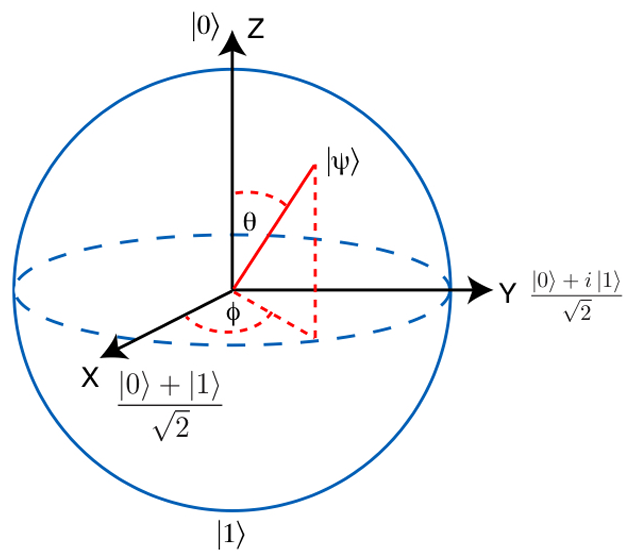
\includegraphics[width=3.5cm, height=3cm]{intro/qubits.png}
    \end{center}

\end{frame}

\begin{frame}
    \begin{theorem}
        The expectation values of the Pauli operators are
        \begin{gather*}
            \langle \sigma_1 \rangle = \sin \theta \cos \phi \,,  \\
            \langle \sigma_2 \rangle = \sin \theta \sin \phi \,, \\
            \langle \sigma_3 \rangle = \cos \theta \,.
        \end{gather*}
    \end{theorem}

\end{frame}

\begin{frame}
    \frametitle{Open system: two qubits}
    Let $A, B$ be two quantum systems. We denote $AB$ to be composite system.
    The Hilbert space $\mathcal{H}_{AB} = \mathcal{H}_A \otimes \mathcal{H}_B$.

    Consider the following state in this system
    \begin{equation*}
        \ket{\Psi}_{AB} = a \ket{0}_A \otimes \ket{0}_B +
                            b \ket{1}_A \otimes \ket{1}_B
                            = a \ket{00} + b\ket{11} \,.
    \end{equation*}
\end{frame}

\begin{frame}
    \frametitle{Open system: two qubits}
    Consider the following observable $A = M_A \otimes I_B$.
    \begin{align*}
        _{AB} \bra{\Psi} M_A \otimes I_B \ket{\Psi}_{AB} 
        &=
        (a^* \bra{00} + b^*\bra{11}) M_A \otimes I_B (a\ket{00} + b\ket{11})\\
        &= \abs{a}^2 \bra{0}M_A \ket{1} + \abs{b}^2 \bra{1} M_A \ket{1} \,.
    \end{align*}
    Rewrite
    \begin{equation*}
        _{AB} \bra{\Psi} M_A \otimes I_B \ket{\Psi}_{AB} 
        =
        \tr(M_A \rho_A)
    \end{equation*}
    where 
    \begin{equation*}
        \rho_A = \abs{a}^2 \ket{0}\bra{0} + \abs{b}^2 \ket{1}\bra{1} 
        = \tr_B( \ket{\Psi} \bra{\Psi})
        = \sum_{i,j,\mu} \psi^*_{j,\mu} \psi_{i,\mu} \ket{i}\bra{j} \,.
    \end{equation*}
    (density operator)
\end{frame}

\begin{frame}
    \frametitle{General case}
    \begin{align*}
        \langle M_A \rangle &= _{AB}\bra{\Psi } M_A \otimes I_B \ket{\Psi}_{AB} \\
                            & = \sum_{j,\nu} a^*_{j\nu} (_A \ket{j}\otimes _B \bra{\nu}) (M_A \otimes I_B)  \sum_{i,\nu} a_{j\nu} (_A \ket{i}\otimes _B \bra{\nu})\\
                            &= \sum_{i,j,\mu} a^*_{j\mu} a_{i,\mu} \bra{j} M_A \ket{i} = \tr (M_A \rho_A) \,.
    \end{align*}
\end{frame}


\begin{frame}
    \frametitle{Properties of density operator}
    \begin{equation*}
        \rho_A 
        = \sum_{i,j,\mu} \psi^*_{j,\mu} \psi_{i,\mu} \ket{i}\bra{j} \,.
    \end{equation*}
    \begin{enumerate}
        \item Hermitian
        \item Non-negative
        \item unit trace
    \end{enumerate}
    Thus, there is an orthonormal basis in which the density operator is diagonal.
    The eigenvalues are non-negative real numbers that sum to one.
    \begin{equation*}
        \rho_A = \sum_i p_i \ket{i}_A \bra{i}_A \,,
    \end{equation*}
    \begin{equation*}
        \sum_i p_i = 1 \,.
    \end{equation*}

\end{frame}

\begin{frame}
If there is just one nonzero eigenvalue, we say the state of $A$ is ``pure''. Otherwise it is ``mixed''.
\end{frame}

\begin{frame}
    \frametitle{Open system: two qubits}
    Why the fuss?

    For $\ket{\Psi}_{AB} = \frac{1}{\sqrt{2}} (\ket{00} + \ket{11})$, we have
    \begin{equation*}
        \rho_A = \frac{1}{2} (\ket{0}\bra{0} + \ket{1}\bra{1}) = \frac{1}{2} I \,.
    \end{equation*}

    If we are in a closed one qubit system
    $\ket{0} = \ket{\uparrow_z}$ and $\ket{1} = \ket{\downarrow_z}$.
    $$\ket{\uparrow_x} = \frac{1}{\sqrt{2}} ( \ket{\uparrow_z} + \ket{\downarrow_z})$$
    $$\ket{\downarrow_x} = \frac{1}{\sqrt{2}} ( \ket{\uparrow_z} - \ket{\downarrow_z})$$
\end{frame}

\begin{frame}
    \frametitle{Open system: two qubits}
    Therefore, when projecting to $\ket{\uparrow_z}$,
    \begin{equation*}
        \frac{1}{\sqrt{2}} (\ket{\uparrow_x} + \ket{\downarrow_x}) 
    \end{equation*}
    becomes $\ket{z}$ with probability 1.

    On the other hand, in an open system
    \begin{equation*}
        \frac{1}{2} (\ket{\uparrow_z}\bra{\uparrow_z} + \ket{\downarrow_z}\bra{\downarrow_z})
        = \frac{1}{2}I.
    \end{equation*}
    Then the projection onto $\ket{\uparrow_z}$ has the expectation value
    \begin{equation*}
        \tr( \ket{\uparrow_z}\bra{\uparrow_z}\rho) = \bra{\uparrow_z }\rho \ket{\uparrow_z} = \frac{1}{2} \,.
    \end{equation*}
\end{frame}


\begin{frame}
    \frametitle{Schmidt decomposition}
    Consider a state in $\mathcal{H}_A\otimes \mathcal{H}_B$
    \begin{equation*}
        \ket{\Psi}_{AB} 
        = \sum_{i,\mu} \psi_{i\mu} \ket{i}_A \otimes \ket{\mu}_B
        \equiv
        \sum_{i} \ket{i}_A \otimes \ket{\tilde i}_B \,,
    \end{equation*}
    where
    \begin{equation*}
        \ket{\tilde i}_B = \sum_\mu \psi_{i\mu} \ket{\mu}_B \,.
    \end{equation*}
\end{frame}


\begin{frame}
    \frametitle{Schmidt decomposition}
    Choose a basis of so that 
    \begin{equation*}
        \rho_A = \sum_i p_i \ket{i}\bra{i} \,.
    \end{equation*}
    Then,
    \begin{equation*}
        \rho_A = \tr_B (\ket{\Psi}\bra{\Psi})
        = \sum_{i,j} \braket{\tilde j}{\tilde i}(\ket{i}\bra{j})
    \end{equation*}
\end{frame}

\begin{frame}
    \frametitle{Schmidt decomposition}
Matching coefficients,
\begin{equation*}
    \braket{\tilde j}{\tilde i}_B = p_i \delta_{ij} \,.
\end{equation*}
Letting
\begin{equation*}
    \ket{i'}_B = p_i^{-1/2} \ket{\tilde i}_B \,,
\end{equation*}
we get
\begin{equation*}
    \ket{\Psi}_{AB} = \sum_i \sqrt{p_i} \ket{i}_A \otimes \ket{i'}_B \,.
\end{equation*}
\end{frame}



\printbibliography 
%\bibliography{refs}
%\bibliographystyle{halpha-abbrv}


\end{document}
